%definira klasu dokumenta 
\documentclass[12pt]{report} 

%prostor izmedu naredbi \documentclass i \begin{document} se zove uvod. U njemu se nalaze naredbe koje se odnose na cijeli dokument

%osnovni LaTex ne može riješiti sve probleme, pa se koriste različiti paketi koji olakšavaju izradu željenog dokumenta
\usepackage[croatian]{babel} 
\usepackage{amssymb}
\usepackage{amsmath}
\usepackage{txfonts}
\usepackage{mathdots}
\usepackage{titlesec}
\usepackage{array}
\usepackage{lastpage}
\usepackage{etoolbox}
\usepackage{tabularray}
\usepackage{color, colortbl}
\usepackage{adjustbox}
\usepackage{geometry}
\usepackage[classicReIm]{kpfonts}
\usepackage{hyperref}
\usepackage{fancyhdr}

\usepackage{float}
\usepackage{setspace}
\restylefloat{table}


\patchcmd{\chapter}{\thispagestyle{plain}}{\thispagestyle{fancy}}{}{} %redefiniranje stila stranice u paketu fancyhdr

%oblik naslova poglavlja
\titleformat{\chapter}{\normalfont\huge\bfseries}{\thechapter.}{20pt}{\Huge}
\titlespacing{\chapter}{0pt}{0pt}{40pt}


\linespread{1.3} %razmak između redaka

\geometry{a4paper, left=1in, top=1in,}  %oblik stranice

\hypersetup{ colorlinks, citecolor=black, filecolor=black, linkcolor=black,	urlcolor=black }   %izgled poveznice


%prored smanjen između redaka u nabrajanjima i popisima
\newenvironment{packed_enum}{
	\begin{enumerate}
		\setlength{\itemsep}{0pt}
		\setlength{\parskip}{0pt}
		\setlength{\parsep}{0pt}
	}{\end{enumerate}}

\newenvironment{packed_item}{
	\begin{itemize}
		\setlength{\itemsep}{0pt}
		\setlength{\parskip}{0pt}
		\setlength{\parsep}{0pt}
	}{\end{itemize}}




%boja za privatni i udaljeni kljuc u tablicama
\definecolor{LightBlue}{rgb}{0.9,0.9,1}
\definecolor{LightGreen}{rgb}{0.9,1,0.9}

%Promjena teksta za dugačke tablice
\DefTblrTemplate{contfoot-text}{normal}{Nastavljeno na idućoj stranici}
\SetTblrTemplate{contfoot-text}{normal}
\DefTblrTemplate{conthead-text}{normal}{(Nastavljeno)}
\SetTblrTemplate{conthead-text}{normal}
\DefTblrTemplate{middlehead,lasthead}{normal}{Nastavljeno od prethodne stranice}
\SetTblrTemplate{middlehead,lasthead}{normal}

%podesavanje zaglavlja i podnožja

\pagestyle{fancy}
\lhead{Programsko inženjerstvo}
\rhead{$<$Projektni zadatak$>$}
\lfoot{$<$Naziv grupe$>$}
\cfoot{stranica \thepage/\pageref{LastPage}}
\rfoot{\today}
\renewcommand{\headrulewidth}{0.2pt}
\renewcommand{\footrulewidth}{0.2pt}


\begin{document} 
	
	
	
	\begin{titlepage}
		\begin{center}
			\vspace*{\stretch{1.0}} %u kombinaciji s ostalim \vspace naredbama definira razmak između redaka teksta
			\LARGE Programsko inženjerstvo\\
			\large Ak. god. 2020./2021.\\
			
			\vspace*{\stretch{3.0}}
			
			\huge Što želiš čitati\\
			\Large Dokumentacija, Rev. \textit{1}\\
			
			\vspace*{\stretch{12.0}}
			\normalsize
			Grupa: \textit{Proggers}\\
			Voditelj: \textit{Sven Winkler}\\
			
			
			\vspace*{\stretch{1.0}}
			Datum predaje: \textit{$<$dan$>$. $<$mjesec$>$. $<$godina$>$.}\\
	
			\vspace*{\stretch{4.0}}
			
			Nastavnik: \textit{Alan Jović}\\
		
		\end{center}

	
	\end{titlepage}

	
	\tableofcontents


	\chapter{Dnevnik promjena dokumentacije}
		
		\textbf{\textit{Kontinuirano osvježavanje}}\\
				
		
		\begin{longtblr}[
				label=none
			]{
				width = \textwidth, 
				colspec={|X[2]|X[13]|X[3]|X[3]|}, 
				rowhead = 1
			}
			\hline
			\textbf{Rev.}	& \textbf{Opis promjene/dodatka} & \textbf{Autori} & \textbf{Datum}\\[3pt] \hline
			0.1 & Napravljen predložak.	& Božidar Pučar & 29.10.2023. 		\\[3pt] \hline 
			0.2	& Dopisane upute za povijest dokumentacije.\newline Dodane reference. & * & 24.08.2013. 	\\[3pt] \hline 
			0.5 & Dodan \textit{Use Case} dijagram i jedan sekvencijski dijagram, funkcionalni i nefunkcionalni zahtjevi i dodatak A & * & 25.08.2013. \\[3pt] \hline 
			0.6 & Arhitektura i dizajn sustava, algoritmi i strukture podataka & * & 26.08.2013. \\[3pt] \hline 
			0.8 & Povijest rada i trenutni status implementacije,\newline Zaključci i plan daljnjeg rada & * & 28.08.2013. \\[3pt] \hline 
			0.9 & Opisi obrazaca uporabe & * & 07.09.2013. \\[3pt] \hline 
			0.10 & Preveden uvod & * & 08.09.2013. \\[3pt] \hline 
			0.11 & Sekvencijski dijagrami & * & 09.09.2013. \\[3pt] \hline 
			0.12.1 & Započeo dijagrame razreda & * & 10.09.2013. \\[3pt] \hline 
			0.12.2 & Nastavak dijagrama razreda & * & 11.09.2013. \\[3pt] \hline 
			\textbf{1.0} & Verzija samo s bitnim dijelovima za 1. ciklus & * & 11.09.2013. \\[3pt] \hline 
			1.1 & Uređivanje teksta -- funkcionalni i nefunkcionalni zahtjevi & * \newline * & 14.09.2013. \\[3pt] \hline 
			1.2 & Manje izmjene:Timer - Brojilo vremena & * & 15.09.2013. \\[3pt] \hline 
			1.3 & Popravljeni dijagrami obrazaca uporabe & * & 15.09.2013. \\[3pt] \hline 
			1.5 & Generalna revizija strukture dokumenta & * & 19.09.2013. \\[3pt] \hline 
			1.5.1 & Manja revizija (dijagram razmještaja) & * & 20.09.2013. \\[3pt] \hline 
			\textbf{2.0} & Konačni tekst predloška dokumentacije  & * & 28.09.2013. \\[3pt] \hline 
			&  &  & \\[3pt] \hline	
		\end{longtblr}
	
	
		\textit{Moraju postojati glavne revizije dokumenata 1.0 i 2.0 na kraju prvog i drugog ciklusa. Između tih revizija mogu postojati manje revizije već prema tome kako se dokument bude nadopunjavao. Očekuje se da nakon svake značajnije promjene (dodatka, izmjene, uklanjanja dijelova teksta i popratnih grafičkih sadržaja) dokumenta se to zabilježi kao revizija. Npr., revizije unutar prvog ciklusa će imati oznake 0.1, 0.2, …, 0.9, 0.10, 0.11.. sve do konačne revizije prvog ciklusa 1.0. U drugom ciklusu se nastavlja s revizijama 1.1, 1.2, itd.}
	\chapter{Opis projektnog zadatka}
		
		\textbf{\textit{dio 1. revizije}}\\
		
		\textit{Na osnovi projektnog zadatka detaljno opisati korisničke zahtjeve. Što jasnije opisati cilj projektnog zadatka, razraditi problematiku zadatka, dodati nove aspekte problema i potencijalnih rješenja. Očekuje se minimalno 3, a poželjno 4-5 stranica opisa.	Teme koje treba dodatno razraditi u ovom poglavlju su:}
		\begin{packed_item}
			\item \textit{potencijalna korist ovog projekta}
			\item \textit{postojeća slična rješenja (istražiti i ukratko opisati razlike u odnosu na zadani zadatak). Dodajte slike koja predočavaju slična rješenja.}
			\item \textit{skup korisnika koji bi mogao biti zainteresiran za ostvareno rješenje.}
			\item \textit{mogućnost prilagodbe rješenja }
			\item \textit{opseg projektnog zadatka}
			\item \textit{moguće nadogradnje projektnog zadatka}
		\end{packed_item}
		
		\textit{Za pomoć pogledati reference navedene u poglavlju „Popis literature“, a po potrebi konzultirati sadržaj na internetu koji nudi dobre smjernice u tom pogledu.}
		\eject
		
		\section{Primjeri u \LaTeX u}
		
		\textit{Ovo potpoglavlje izbrisati.}\\

		U nastavku se nalaze različiti primjeri kako koristiti osnovne funkcionalnosti \LaTeX a koje su potrebne za izradu dokumentacije. Za dodatnu pomoć obratiti se asistentu na projektu ili potražiti upute na sljedećim web sjedištima:
		\begin{itemize}
			\item Upute za izradu diplomskog rada u \LaTeX u - \url{https://www.fer.unizg.hr/_download/repository/LaTeX-upute.pdf}
			\item \LaTeX\ projekt - \url{https://www.latex-project.org/help/}
			\item StackExchange za Tex - \url{https://tex.stackexchange.com/}\\
		
		\end{itemize} 	


		
		\noindent \underbar{podcrtani tekst}, \textbf{podebljani tekst}, 	\textit{nagnuti tekst}\\
		\noindent \normalsize primjer \large primjer \Large primjer \LARGE {primjer} \huge {primjer} \Huge primjer \normalsize
				
		\begin{packed_item}
			
			\item  primjer
			\item  primjer
			\item  primjer
			\item[] \begin{packed_enum}
				\item primjer
				\item[] \begin{packed_enum}
					\item[1.a] primjer
					\item[b] primjer
				\end{packed_enum}
				\item primjer
			\end{packed_enum}
			
		\end{packed_item}
		
		\noindent primjer url-a: \url{https://www.fer.unizg.hr/predmet/proinz/projekt}
		
		\noindent posebni znakovi: \# \$ \% \& \{ \} \_ 
		$|$ $<$ $>$ 
		\^{} 
		\~{} 
		$\backslash$ 
		
		
		\begin{longtblr}[
			label=none,
			entry=none
			]{
				width = \textwidth,
				colspec={|X[8,l]|X[8, l]|X[16, l]|}, 
				rowhead = 1,
			} %definicija širine tablice, širine stupaca, poravnanje i broja redaka naslova tablice
			\hline \SetCell[c=3]{c}{\textbf{naslov unutar tablice}}	 \\ \hline[3pt]
			\SetCell{LightGreen}IDKorisnik & INT	&  	Lorem ipsum dolor sit amet, consectetur adipiscing elit, sed do eiusmod  	\\ \hline
			korisnickoIme	& VARCHAR &   	\\ \hline 
			email & VARCHAR &   \\ \hline 
			ime & VARCHAR	&  		\\ \hline 
			\SetCell{LightBlue} primjer	& VARCHAR &   	\\ \hline 
		\end{longtblr}
		

		\begin{longtblr}[
				caption = {Naslov s referencom izvan tablice},
				entry = {Short Caption},
			]{
				width = \textwidth, 
				colspec = {|X[8,l]|X[8,l]|X[16,l]|}, 
				rowhead = 1,
			}
			\hline
			\SetCell{LightGreen}IDKorisnik & INT	&  	Lorem ipsum dolor sit amet, consectetur adipiscing elit, sed do eiusmod  	\\ \hline
			korisnickoIme	& VARCHAR &   	\\ \hline 
			email & VARCHAR &   \\ \hline 
			ime & VARCHAR	&  		\\ \hline 
			\SetCell{LightBlue} primjer	& VARCHAR &   	\\ \hline 
		\end{longtblr}
	


		
		
		%unos slike
		\begin{figure}[H]
			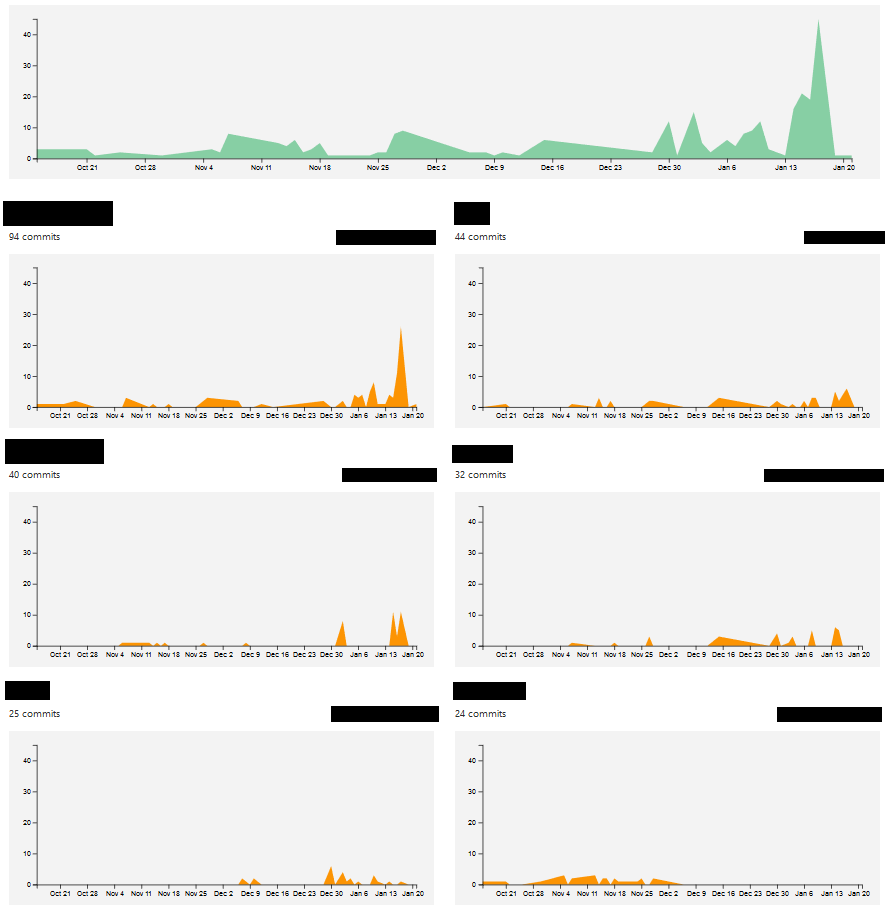
\includegraphics[scale=0.4]{slike/aktivnost.PNG} %veličina slike u odnosu na originalnu datoteku i pozicija slike
			\centering
			\caption{Primjer slike s potpisom}
			\label{fig:promjene}
		\end{figure}
		
		\begin{figure}[H]
			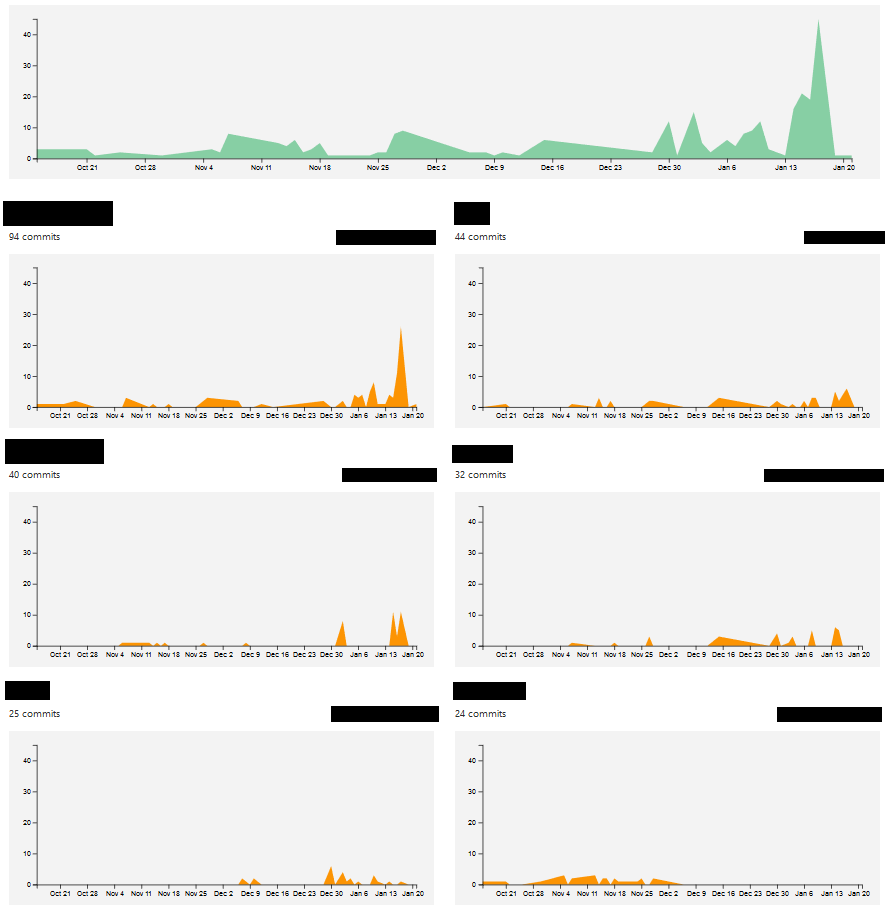
\includegraphics[width=\textwidth]{slike/aktivnost.PNG} %veličina u odnosu na širinu linije
			\caption{Primjer slike s potpisom 2}
			\label{fig:promjene2} %label mora biti drugaciji za svaku sliku
		\end{figure}
		
		Referenciranje slike \ref{fig:promjene2} u tekstu.
		
		\eject
		
	
	\documentclass[12pt]{report}  

\usepackage[croatian]{babel} 
\usepackage{amssymb}
\usepackage{amsmath}
\usepackage{txfonts}
\usepackage{mathdots}
\usepackage{titlesec}
\usepackage{array}
\usepackage{lastpage}
\usepackage{etoolbox}
\usepackage{tabularray}
\usepackage{color, colortbl}
\usepackage{adjustbox}
\usepackage{geometry}
\usepackage[classicReIm]{kpfonts}
\usepackage{hyperref}
\usepackage{fancyhdr}

\usepackage{float}
\usepackage{setspace}
\restylefloat{table}

\begin{document}
\setcounter{chapter}{2}
\chapter{Specifikacija programske potpore}

\section{Funkcionalni zahtjevi}

\noindent \textbf{Dionici:}

\begin{enumerate}
	
	\item Kupci 
	\item Ponuditelji
	\begin{enumerate}
		\item Izdavač
		\item Antikvarijat
		\item Preprodavač
	\end{enumerate}	
	\item Administrator		
	\item Razvojni tim
	
\end{enumerate}

\noindent \textbf{Aktori i njihovi funkcionalni zahtjevi:}


\begin{enumerate}
	\item  \underbar{Neregistrirani korisnik (inicijator) može:}
	
	\begin{enumerate}
		
		\item pretraživati ponude knjiga
		\begin{enumerate}
			
			\item  po značajkama knjige (naziv, autori, godina izdanja, izdavač,
			kategorija izdavača (domaći, strani), žanr, ISBN, broj izdanja, stanje očuvanosti,
			tekstni opis, slika korica, oznaka vrste knjige i lista ponuda)
			\item  po nazivu ponuditelja (izlistati sve knjige dotičnog)
			\item na karti (npr. OpenStreetMap) gdje su označene lokacije svih ponuditelja knjiga
			
		\end{enumerate}
		\item  zatražiti od izdavača da kontaktira stranog izdavača oko prijevoda strane knjige na hrvatski jezik
		
		\item vidjeti popis dostupnih ponuda za odabranu knjigu, uključujući naziv ponuditelja, broj dostupnih primjeraka i cijenu knjige kod svakog ponuditelja
		
		
		
	\end{enumerate}
	
	\item  \underbar{Svaki ponuditelj (izdavač, antikvarijat, preprodavač) (inicijator) može:}
	
	\begin{enumerate}
		
		\item ponuditi neograničeni broj naslova knjiga i primjeraka knjiga
		\item uklanjati primjerke već postojeće knjige 
		
	\end{enumerate}
	
	\item \underbar{Izdavač (inicijator) može:}
	
	zatražiti izdavača strane knjige za dozvolu prijevoda knjige sa stranog ili srodnog jezika na hrvatski jezik
	
	\item \underbar{Antikvarijat (inicijator) može:}
	
	nuditi knjige na stranom jeziku, srodnom jeziku ili hrvatskom jeziku
	
	
	\item \underbar{Preprodavač (inicijator) može:}
	
	nuditi sve vrste knjiga, uključujući i one koje nisu na drugačiji način dobavljive na području
	Hrvatske
	
	\item \underbar{Administrator (inicijator) može:}
	\begin{enumerate}
		\item odobriti registracije ponuditelja
		\item upravljati korisničkim računima
		\item riješavati sporove i pratiti komunikaciju između neregistriranih korisnika i ponuditelja
	\end{enumerate}
		
	\item \underbar{Baza podataka (sudionik):}
	
	\begin{enumerate}
		
		\item pohranjuje sve podatke o korisnicima i njihovim ovlastima
		
		\item pohranjuje sve podatke o knjigama kao i zahtjeve za prijevod za svaku knjigu na stranom jeziku
		
	\end{enumerate}
	
\end{enumerate}

\eject 



\subsection{Obrasci uporabe}

\subsubsection{Opis obrazaca uporabe}

\noindent \underbar{\textbf{UC1 - Pregled knjiga na karti}}
\begin{enumerate}
	
	\item \textbf{Glavni sudionik: }Neregistrirani korisnik
	\item  \textbf{Cilj:} Pregledati dostupne knjige uz pomoć karte
	\item  \textbf{Sudionici:} Baza podataka
	\item  \textbf{Preduvjet:} - 
	\item  \textbf{Opis osnovnog tijeka:}
	
	\begin{enumerate}
		
		\item Karta je prikazana prilikom učitavanja aplikacije
		\item Neregistrirani korisnik odabire ponuditelja na karti
		\item Izlistavaju se sve knjige dotičnog ponuditelja
		
	\end{enumerate}

\end{enumerate}


\noindent \underbar{\textbf{UC2 - Registracija}}
\begin{enumerate}
	
	\item \textbf{Glavni sudionik: }Neregistrirani korisnik
	\item  \textbf{Cilj:} Stvoriti korisnički račun za pristup sustavu 
	\item  \textbf{Sudionici:} Baza podataka
	\item  \textbf{Preduvjet:} - 
	\item  \textbf{Opis osnovnog tijeka:}
	
	\begin{enumerate}
		
		\item Korisnik odabire opciju za registraciju
		\item Korisnik unosi potrebne korisničke podatke i bira između 3 navedene vrste ponuditelja
		\item Korisnik prima obavijest o uspješnoj registraciji nakon administratorskog pregleda
		
	\end{enumerate}
	
		
	\item  \textbf{Opis mogućih odstupanja:}
	
	\item[] \begin{enumerate}
		
		\item[2.a] Odabir već zauzetog korisničkog imena i/ili e-maila, unos korisničkog
		podatka u nedozvoljenom formatu ili pružanje neispravnoga e-maila ili odabir adrese koja se ne podudara sa pravilima aplikacije
		\item[] \begin{enumerate}
			
			\item Sustav obavještava korisnika o neuspjelom upisu i vraća ga na stra-
			nicu za registraciju
			\item Korisnik mijenja potrebne podatke te završava unos ili odustaje od registracije
			
		\end{enumerate}
		
	\end{enumerate}
	
\end{enumerate}

\noindent \underbar{\textbf{UC3 - Prijava u sustav}}
\begin{enumerate}
	
	\item \textbf{Glavni sudionik: } Ponuditelj
	\item  \textbf{Cilj:} Autentifikacija korisnika
	\item  \textbf{Sudionici:} Baza podataka
	\item  \textbf{Preduvjet:} Registracija
	\item  \textbf{Opis osnovnog tijeka:}
	
	\begin{enumerate}
		
		\item Unos korisničkog imena i lozinke
		\item Potvrda o ispravnosti unesenih podataka
		\item Pristup funkcijama registriranih korisnika, ovisno o tipu ponuditelja
		
	\end{enumerate}
	
	\item  \textbf{Opis mogućih odstupanja:}
	
	\item[] \begin{enumerate}
		
		\item[2.a] Neispravno korisničko ime/lozinka
		\item[] \begin{enumerate}
			
			\item Sustav obavještava korisnika o neuspjelom upisu i vraća ga na stra-
			nicu za prijavu
			
		\end{enumerate}
		
	\end{enumerate}
	
\end{enumerate}

\noindent \underbar{\textbf{UC4 - Pretraživanje knjiga po značajkama knjige}}
\begin{enumerate}
	
	\item \textbf{Glavni sudionik: } Neregistrirani korisnik
	\item  \textbf{Cilj:} Pronalazak željene knjige
	\item  \textbf{Sudionici:} Baza podataka
	\item  \textbf{Preduvjet:} -
	\item  \textbf{Opis osnovnog tijeka:}
	
	\begin{enumerate}
		
		\item Unos značajki knjige u odgovarajuće polje
		\item Izlistavanje knjiga koje se podudaraju sa tim značajkama
		
	\end{enumerate}
	
	\item  \textbf{Opis mogućih odstupanja:}
	
	\item[] \begin{enumerate}
		
		\item[2.a] Nepodudaranje sa ijednom knjigom u bazi podataka
		\item[] \begin{enumerate}
			
			\item Sustav obavještava korisnika o tome da knjiga ili ne postoji ili nije dostupna
			
		\end{enumerate}
		
	\end{enumerate}
	
\end{enumerate}

\noindent \underbar{\textbf{UC5 - Pretraživanje knjiga po nazivu ponuditelja}}
\begin{enumerate}
	
	\item \textbf{Glavni sudionik: } Neregistrirani korisnik
	\item  \textbf{Cilj:} Izlistavanje knjiga određenog ponuditelja
	\item  \textbf{Sudionici:} Baza podataka
	\item  \textbf{Preduvjet:} -
	\item  \textbf{Opis osnovnog tijeka:}
	
	\begin{enumerate}
		
		\item Unos naziva ponuditelja u odgovarajuće polje
		\item Izlistavanje knjiga koje su na ponuditeljevom popisu
		
	\end{enumerate}
	
	\item  \textbf{Opis mogućih odstupanja:}
	
	\item[] \begin{enumerate}
		
		\item[2.a] Nepodudaranje sa ijednim ponuditeljem u bazi podataka
		\item[] \begin{enumerate}
			
			\item Sustav obavještava korisnika o tome da ponuditelj ili ne postoji ili nema nijednu knjigu na trenutnoj ponudi
			
		\end{enumerate}
		
	\end{enumerate}
	
\end{enumerate}

\noindent \underbar{\textbf{UC6 - Zatražiti izdavača da kontaktira stranog izdavača oko prijevoda strane knjige na hrvatski jezik}}
\begin{enumerate}
	
	\item \textbf{Glavni sudionik: } Neregistrirani korisnik
	\item  \textbf{Cilj:} Zatražiti prijevod strane knjige na hrvatski jezik
	\item  \textbf{Sudionici:} Baza podataka
	\item  \textbf{Preduvjet:} Izdavač postoji i pronađen je kroz search
	\item  \textbf{Opis osnovnog tijeka:}
	
	\begin{enumerate}
	 
		\item Neregistrirani korisnik upiše značajke strane knjige
		\item Sustav obavještava korisnika da je upit poslan
		
	\end{enumerate}
	
\end{enumerate}

\noindent \underbar{\textbf{UC7 - Dodavanje knjige}}
\begin{enumerate}
	
	\item \textbf{Glavni sudionik: } Ponuditelj
	\item  \textbf{Cilj:} Dodati dostupnu knjigu 
	\item  \textbf{Sudionici:} Baza podataka
	\item  \textbf{Preduvjet:} Ponuditelj je prijavljen u sustav
	\item  \textbf{Opis osnovnog tijeka:}
	
	\begin{enumerate}
		
		\item Ponuditelj odabere opciju za dodavanje primjerka knjige
		\item Ponuditelj upisuje sve značajke knjige   
		\item Potvrda o upisu knjige u bazu podataka kao nove knjige ili kao još jedan primjerak već postojeće
		
	\end{enumerate}
	
\end{enumerate}

\noindent \underbar{\textbf{UC8 - Uklanjanje knjige}}
\begin{enumerate}
	
	\item \textbf{Glavni sudionik: } Ponuditelj
	\item  \textbf{Cilj:} Izbrisati primjerak knjige
	\item  \textbf{Sudionici:} Baza podataka
	\item  \textbf{Preduvjet:} Ponuditelj je prijavljen u sustav
	\item  \textbf{Opis osnovnog tijeka:}
	
	\begin{enumerate}
		
		\item Ponuditelj odabere opciju za brisanje primjerka knjige
		\item Ponuditelj upisuje sve značajke knjige 
		\item Potvrda o smanjenju primjeraka knjige 
		
	\end{enumerate}
	
	\item  \textbf{Opis mogućih odstupanja:}
	
	\item[] \begin{enumerate}
		
		\item[2.a] Ponuditelj nije niti nudio knjigu ili je već na 0 primjeraka 
		\item[] \begin{enumerate}
			
			\item Sustav obavještava ponuditelja o nemogućnosti uklanjanja primjerka određene knjige
			
		\end{enumerate}
		
	\end{enumerate}
	
\end{enumerate}

\noindent \underbar{\textbf{UC9 - Uređivanje knjige}}
\begin{enumerate}
	
	\item \textbf{Glavni sudionik: } Ponuditelj
	\item  \textbf{Cilj:} Urediti knjigu
	\item  \textbf{Sudionici:} Baza podataka
	\item  \textbf{Preduvjet:} Ponuditelj je prijavljen u sustav
	\item  \textbf{Opis osnovnog tijeka:}
	
	\begin{enumerate}
		
		\item Ponuditelj odabere opciju za uređivanje knjige
		\item Ponuditelj upisuje promjene značajke knjige 
		\item Ponuditelj sprema promjene
		\item Sustav potvrđuje promjene
		
	\end{enumerate}
	
	\item  \textbf{Opis mogućih odstupanja:}
	
	\item[] \begin{enumerate}
		
		\item[2.a] Ponuditelj nije niti nudio knjigu ili je već na 0 primjeraka 
		\item[] \begin{enumerate}
			
			\item Sustav obavještava ponuditelja o nemogućnosti uklanjanja primjerka određene knjige
			
		\end{enumerate}
		
	\end{enumerate}
	
\end{enumerate}

\noindent \underbar{\textbf{UC10 - Neregistrirani korisnik vidi podatke za odabranu knjigu}}
\begin{enumerate}
	
	\item \textbf{Glavni sudionik: } Ponuditelj
	\item  \textbf{Cilj:} 
	\item  \textbf{Sudionici:} Baza podataka
	\item  \textbf{Preduvjet:} Knjiga postoji u bazi podataka
	\item  \textbf{Opis osnovnog tijeka:}
	
	\begin{enumerate}
		
		\item Neregistrirani korisnik klikne na knjigu 
		\item Ispisuje se popis dostupnih ponuda za odabranu knjigu, uključujući naziv ponuditelja, broj dostupnih primjeraka i cijenu knjige kod svakog ponuditelja.
		\item Potvrda o smanjenju primjeraka knjige 
		
	\end{enumerate}
	
	\item  \textbf{Opis mogućih odstupanja:}
	
	\item[] \begin{enumerate}
		
		\item[2.a] Ponuditelj nije niti nudio knjigu ili je već na 0 primjeraka 
		\item[] \begin{enumerate}
			
			\item Sustav obavještava ponuditelja o nemogućnosti uklanjanja primjerka određene knjige
			
		\end{enumerate}
		
	\end{enumerate}
	
\end{enumerate}

\section{Ostali zahtjevi}
\begin{itemize}
	\item Sustav treba podržavati rad više korisnika u stvarnom vremenu
	\item Ponuditelj može dodati bilo koju knjigu za koju želi da bude ponuđena u aplikaciji, a drugim kanalima može nuditi neke druge knjige
	\item Komunikacija neregistriranih korisnika (onih koji traže neku knjigu) i ponuditelja ne odvija se kroz aplikaciju, već za to služe drugi kanali komunikacije (npr. e-pošta, telefon)
	\item Korisničko sučelje i sustav moraju podržavati hrvatsku abecedu (dijakritičke znakove) pri unosu i prikazu tekstualnog sadržaja
	\item Aplikacija treba biti izvedena kao web aplikacija prilagođena (engl. Responsive) mobilnom uređaju ili tabletu
	\item Registrirani korisnici trebaju joj pristupati uz pomoć korisničkog imena i lozinke
	\item Nadogradnja sustava ne smije narušavati postojeće funkcionalnosti sustava
\end{itemize}



\end{document}

	\chapter{Arhitektura i dizajn sustava}

Kako bi se omogućio ispravan rad web aplikacije te interakcija između korisnika i nje potrebno je nekoliko osnovnih komponenata. To su:

	\begin{itemize}
		\item \textbf{Web preglednik}
		\item \textbf{Web aplikacija}
		\item \textbf{Web poslužitelj}
		\item \textbf{Baza podataka i njezin poslužitelj}		
	\end{itemize}

	\begin{figure}[H]
		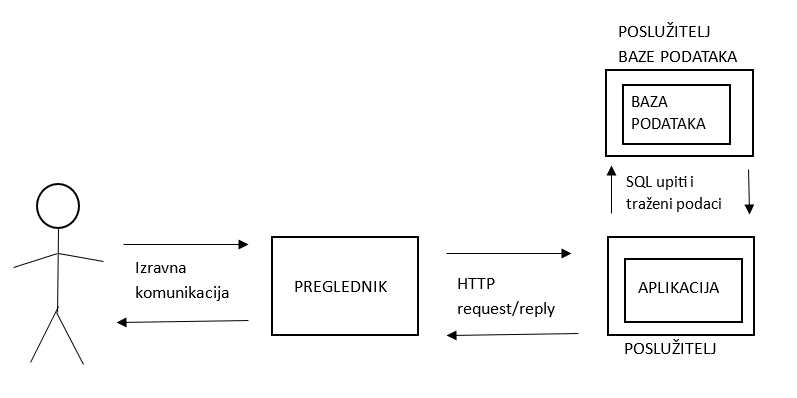
\includegraphics[scale=0.4]{slike/komunikacijaKomponenata.PNG}
		\centering
		\caption{Prikaz komunikacije između navedenih dijelova sustava}
		\label{fig:skicaKomunijacije}
	\end{figure}

	
	Web preglednik (klijent) šalje zahtjeve poslužitelju te prima odgovore kako bi prikazao sadržaj potreban korisniku. Nakon što dohvati programski kod te označni (markup) tekst potreban za prikaz web stranice, on prevodi taj kod i prikazuje ga korisniku na unaprijed definiran način. Način na koji će preglednik prikazati određeni element ili strukturu markup teksta nije propisan samim markup kodom, već ga određuje sam preglednik. Osim osnovnog koda stranice (.html), preglednik dohvaća i .css i .js datoteke te multimedijske sadržaje kao što su slike, videozapisi, zvuk i sl. \vspace{\baselineskip}
	
Sama komunikacija između preglednika i poslužitelja odvija se protokolom HTTP (Hypertext transfer protokol). Nakon što poslužitelj primi HTTP zahtjev, prosljeđuje ga web aplikaciji koja ga zatim obrađuje. Rezultat obrade se, nakon toga, vraća poslužitelju, koji ga prosljeđuje natrag korisniku u obliku HTTP odgovora. Tijekom obrade zahtjeva, ovisno o njegovoj prirodi, web aplikacija ponekad treba pristupiti bazi podataka. Bazi podataka se pristupa putem upita (npr. SQL). Koristit ćemo relacijsku bazu podataka i sustav PostgreSQL. Naime, s navedenom vrstom baza smo najbolje upoznati i imamo najviše iskustva u radu s njima. Osim toga, smatramo da nam omogućava ostvarenje svih planiranih funkcionalnosti potrebnih za našu aplikaciju. PostgreSQL se također temelji na modelu klijent – poslužitelj. Poslužitelj je u ovom slučaju povezan s bazom podataka te prima upite koje šalje web aplikacija. Server ih procesuira, pribavlja tražene informacije iz baze podataka te ih šalje aplikaciji. Aplikacija tada može dovršiti započetu operaciju tj. obraditi zahtjev korisnika/preglednika. \vspace{\baselineskip}

Za izradu aplikacije koristit ćemo programski jezik Java. Naime, to je jezik s kojim je većina članova našeg tima najbolje upoznata. Kako bismo ostvarili funkcionalnost backenda za našu aplikaciju, uz programski jezik Java koristit ćemo Spring radni okvir (framework). Za frontend ćemo koristiti JavaScript i njegov React library koji će nam omogućiti jednostavniju i elegantniju izradu web stranice. \vspace{\baselineskip}

Arhitektura sustava temeljit će se na MVC konceptu (model-controller-view). Ovaj način razvoja aplikacije ima brojne prednosti, ponajviše glede odvojenog razvoja dijelova aplikacije. S obzirom na to da su odgovornosti razdvojene kad se primjenjuje ova arhitektura, mnogo je lakše zasebno razvijati svaki dio te ga testirati odvojeno od ostalih. Olakšano je pronalaženje pogrešaka u programskom kodu te vršenje izmjena nad postojećim dijelovima projekta, bez većeg kompromitiranja postojećih funkcionalnosti. Osim toga, ovakav pristup olakšao bi rad na skalabilnosti aplikacije, ako bi to bilo potrebno u bilo kojem trenutku. Još jedan od razloga za korištenje arhitekture temeljene na MVC načelu je činjenica da ju podržava Spring radni okvir koji koristimo. Dijelovi ove arhitekture su sljedeći:

\begin{itemize}
\item \textbf{Model} – obuhvaća logiku i funkcionalnost aplikacije u smislu obrade podataka i upravljanja istima. Prima podatke od controllera i na temelju toga izvršava potrebne radnje nad podatcima te vraća rezultat natrag.

\item \textbf{Controller} – poveznica između model i view komponenata. Prihvaća zahtjeve poslane od strane korisnika te određuje kako odgovoriti na njih. Te informacije prosljeđuje modelu. Kad od modela dobije odgovor, rezultat obrade vraća korisniku putem view komponente. Podatci koje controller dobiva od korisnika mogu biti klikovi na gumbe, poslani obrasci i sl.

\item \textbf{View} – odnosi se na front end stranu aplikacije. To su dijelovi aplikacije koje korisnik vidi i s kojima izravno komunicira. View pribavlja podatke od modela te ih prikazuje na zaslonu računala na način razumljiv čovjeku. To su HTML, CSS datoteke i JS skripte na strani klijenta. 
\end{itemize}

		

				
		\section{Baza podataka}
			
			\textbf{\textit{dio 1. revizije}}\\
			
		\textit{Potrebno je opisati koju vrstu i implementaciju baze podataka ste odabrali, glavne komponente od kojih se sastoji i slično.}
		
			\subsection{Opis tablica}
			

				\textit{Svaku tablicu je potrebno opisati po zadanom predlošku. Lijevo se nalazi točno ime varijable u bazi podataka, u sredini se nalazi tip podataka, a desno se nalazi opis varijable. Svjetlozelenom bojom označite primarni ključ. Svjetlo plavom označite strani ključ}
				
				
				\begin{longtblr}[
					label=none,
					entry=none
					]{
						width = \textwidth,
						colspec={|X[6,l]|X[6, l]|X[20, l]|}, 
						rowhead = 1,
					} %definicija širine tablice, širine stupaca, poravnanje i broja redaka naslova tablice
					\hline \SetCell[c=3]{c}{\textbf{korisnik - ime tablice}}	 \\ \hline[3pt]
					\SetCell{LightGreen}IDKorisnik & INT	&  	Lorem ipsum dolor sit amet, consectetur adipiscing elit, sed do eiusmod  	\\ \hline
					korisnickoIme	& VARCHAR &   	\\ \hline 
					email & VARCHAR &   \\ \hline 
					ime & VARCHAR	&  		\\ \hline 
					\SetCell{LightBlue} primjer	& VARCHAR &   	\\ \hline 
				\end{longtblr}
				
				
			
			\subsection{Dijagram baze podataka}
				\textit{ U ovom potpoglavlju potrebno je umetnuti dijagram baze podataka. Primarni i strani ključevi moraju biti označeni, a tablice povezane. Bazu podataka je potrebno normalizirati. Podsjetite se kolegija "Baze podataka".}
			
			\eject
			
			
		\section{Dijagram razreda}
		
			\textit{Potrebno je priložiti dijagram razreda s pripadajućim opisom. Zbog preglednosti je moguće dijagram razlomiti na više njih, ali moraju biti grupirani prema sličnim razinama apstrakcije i srodnim funkcionalnostima.}\\
			
			\textbf{\textit{dio 1. revizije}}\\
			
			\textit{Prilikom prve predaje projekta, potrebno je priložiti potpuno razrađen dijagram razreda vezan uz \textbf{generičku funkcionalnost} sustava. Ostale funkcionalnosti trebaju biti idejno razrađene u dijagramu sa sljedećim komponentama: nazivi razreda, nazivi metoda i vrste pristupa metodama (npr. javni, zaštićeni), nazivi atributa razreda, veze i odnosi između razreda.}\\
			
			\textbf{\textit{dio 2. revizije}}\\			
			
			\textit{Prilikom druge predaje projekta dijagram razreda i opisi moraju odgovarati stvarnom stanju implementacije}
			
			
			
			\eject
		
		\section{Dijagram stanja}
			
			
			\textbf{\textit{dio 2. revizije}}\\
			
			\textit{Potrebno je priložiti dijagram stanja i opisati ga. Dovoljan je jedan dijagram stanja koji prikazuje \textbf{značajan dio funkcionalnosti} sustava. Na primjer, stanja korisničkog sučelja i tijek korištenja neke ključne funkcionalnosti jesu značajan dio sustava, a registracija i prijava nisu. }
			
			
			\eject 
		
		\section{Dijagram aktivnosti}
			
			\textbf{\textit{dio 2. revizije}}\\
			
			 \textit{Potrebno je priložiti dijagram aktivnosti s pripadajućim opisom. Dijagram aktivnosti treba prikazivati značajan dio sustava.}
			
			\eject
		\section{Dijagram komponenti}
		
			\textbf{\textit{dio 2. revizije}}\\
		
			 \textit{Potrebno je priložiti dijagram komponenti s pripadajućim opisom. Dijagram komponenti treba prikazivati strukturu cijele aplikacije.}
	\chapter{Implementacija i korisničko sučelje}
		
		
		\section{Korištene tehnologije i alati}
			 		
			Komunikacija unutar tima ostvaruje se korištenjem popularnih aplikacija, kao što su \textbf{WhatsApp}$^{[1]}$ i \textbf{Discord}$^{[2]}$. Za modeliranje UML dijagrama koristili smo \textbf{Astah UML}$^{[3]}$,  \textbf{draw.io}$^{[4]}$ te \textbf{ERDPlus}$^{[5]}$ (za ER dijagrame baze podataka). 
			
			\textbf{Git}$^{[6]}$ je centralni sustav za upravljanje izvornim kodom, a projektni udaljeni repozitorij dostupan je na web platformi \textbf{GitHub}$^{[7]}$.
			
			Razvoj frontend-a izveden je u \textbf{JavaScriptu}$^{[8]}$ koristeći biblioteku \textbf{React}$^{[9]}$ koja je održavana od strane Facebooka. Za uređivanje koda koristili smo Microsftov uređivač koda \textbf{Visual Studio Code (VSCode)}$^{[10]}$, koji pruža izvrsnu podršku za razvoj modernih web aplikacija.
			
			Za backend, koristili smo \textbf{IntelliJ IDEA}$^{[11]}$, integrirano razvojno okruženje (IDE) tvrtke JetBrains. IntelliJ pruža snažnu potporu za razvoj Java Spring aplikacija.
			
			Baza podataka koju koristimo je \textbf{PostgreSQL}$^{[12]}$. PostgreSQL je snažan open-source sustav za upravljanje bazama podataka. Za lokalno testiranje baze podataka koristimo \textbf{pgAdmin 4}$^{[13]}$, korisničko sučelje za PostgreSQL bazu podataka.
			
			Pogon aplikacije vršimo putem \textbf{Render}$^{[14]}$ platforme, koja omogućava jednostavan i efikasan proces. Render pruža usluge poput web hostinga, skaliranja aplikacija i upravljanja resursima u oblaku.
			
			Za dokumentaciju koristimo \textbf{TeXstudio}$^{[15]}$ koji podržava LaTeX. LaTeX je sistem za pripremu dokumenata koji se koristi za visokokvalitetno formatiranje tekstova.
			
			Za testiranje i razvoj API-ja koristili smo alat \textbf{Postman}$^{[16]}$, koji pojednostavljuje proces rada s API-ima, omogućujući slanje, testiranje i dokumentiranje HTTP zahtjeva.
			
			$^{1}$\url{https://www.whatsapp.com/}
			
			$^{2}$\url{https://discord.com/}
			
			$^{3}$\url{https://astah.net/products/astah-uml/}
			
			$^{4}$\url{https://www.drawio.com/}
			
			$^{5}$\url{https://erdplus.com/}
			
			$^{6}$\url{https://git-scm.com/}
			
			$^{7}$\url{https://github.com/}
			
			$^{8}$\url{https://www.javascript.com/}
			
			$^{9}$\url{https://reactjs.org/}
			
			$^{10}$\url{https://code.visualstudio.com/}
			
			$^{11}$\url{https://www.jetbrains.com/idea/}
			
			$^{12}$\url{https://www.postgresql.org/}
			
			$^{13}$\url{https://www.pgadmin.org/}
			
			$^{14}$\url{https://render.com/}
			
			$^{15}$\url{https://www.texstudio.org/}
			
			$^{16}$\url{https://www.postman.com/}
			
			\eject 
		
	
		\section{Ispitivanje programskog rješenja}
			
			\textbf{\textit{dio 2. revizije}}\\
			
			 \textit{U ovom poglavlju je potrebno opisati provedbu ispitivanja implementiranih funkcionalnosti na razini komponenti i na razini cijelog sustava s prikazom odabranih ispitnih slučajeva. Studenti trebaju ispitati temeljnu funkcionalnost i rubne uvjete.}
	
			
			\subsection{Ispitivanje komponenti}
			\textit{Potrebno je provesti ispitivanje jedinica (engl. unit testing) nad razredima koji implementiraju temeljne funkcionalnosti. Razraditi \textbf{minimalno 6 ispitnih slučajeva} u kojima će se ispitati redovni slučajevi, rubni uvjeti te izazivanje pogreške (engl. exception throwing). Poželjno je stvoriti i ispitni slučaj koji koristi funkcionalnosti koje nisu implementirane. Potrebno je priložiti izvorni kôd svih ispitnih slučajeva te prikaz rezultata izvođenja ispita u razvojnom okruženju (prolaz/pad ispita). }
			
			
			
			\subsection{Ispitivanje sustava}
			
			 \textit{Potrebno je provesti i opisati ispitivanje sustava koristeći radni okvir Selenium\footnote{\url{https://www.seleniumhq.org/}}. Razraditi \textbf{minimalno 4 ispitna slučaja} u kojima će se ispitati redovni slučajevi, rubni uvjeti te poziv funkcionalnosti koja nije implementirana/izaziva pogrešku kako bi se vidjelo na koji način sustav reagira kada nešto nije u potpunosti ostvareno. Ispitni slučaj se treba sastojati od ulaza (npr. korisničko ime i lozinka), očekivanog izlaza ili rezultata, koraka ispitivanja i dobivenog izlaza ili rezultata.\\ }
			 
			 \textit{Izradu ispitnih slučajeva pomoću radnog okvira Selenium moguće je provesti pomoću jednog od sljedeća dva alata:}
			 \begin{itemize}
			 	\item \textit{dodatak za preglednik \textbf{Selenium IDE} - snimanje korisnikovih akcija radi automatskog ponavljanja ispita	}
			 	\item \textit{\textbf{Selenium WebDriver} - podrška za pisanje ispita u jezicima Java, C\#, PHP koristeći posebno programsko sučelje.}
			 \end{itemize}
		 	\textit{Detalji o korištenju alata Selenium bit će prikazani na posebnom predavanju tijekom semestra.}
			
			\eject 
		
		
		\section{Dijagram razmještaja}
			
			
			 Slika \ref{fig:DijRazm} prikazuje odnos komponenti u sustavu. Klijent preko svog Korisničkog uređaja putem Web preglednika pirstupa Poslužitelju putem HTTP protokola. Poslužitelj se sastoji od Web apliakcije koja izvlači podatke iz baze podataka te zato ovisi o njoj.
			 
			 \begin{figure}[H]
			 	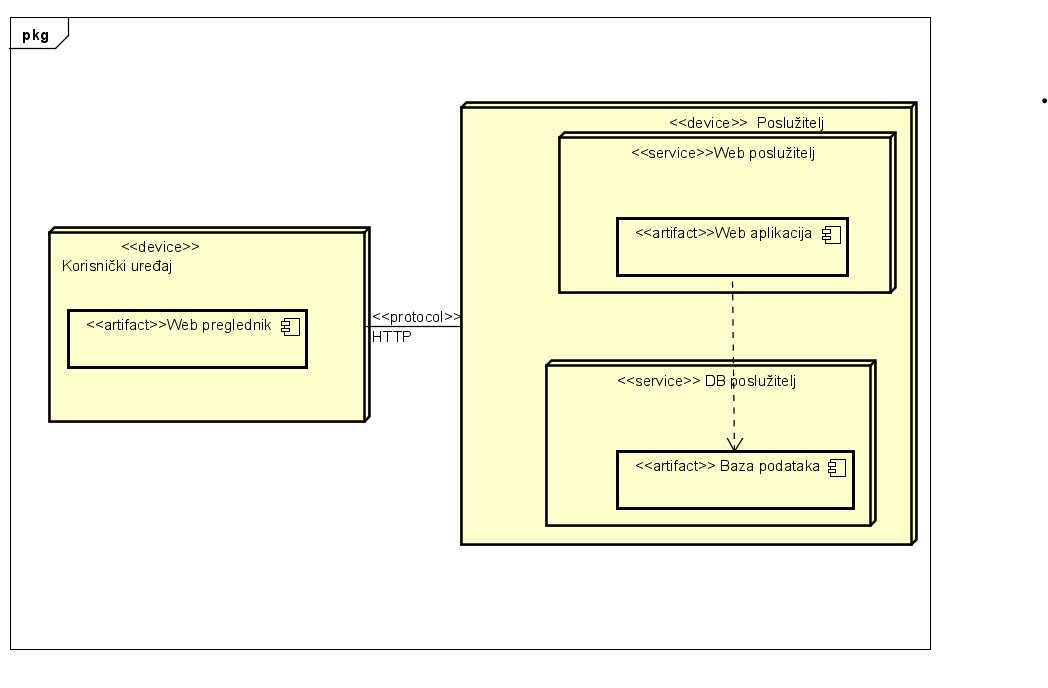
\includegraphics[scale=0.4]{slike/dijagramRaz.jpeg} %veličina slike u odnosu na originalnu datoteku i pozicija slike
			 	\centering
			 	\caption{Dijagram Razmještaja}
			 	\label{fig:DijRazm}
			 \end{figure}
			
			\eject 
		
		\section{Upute za puštanje u pogon}
		
			\textbf{\textit{dio 2. revizije}}\\
		
			 \textit{U ovom poglavlju potrebno je dati upute za puštanje u pogon (engl. deployment) ostvarene aplikacije. Na primjer, za web aplikacije, opisati postupak kojim se od izvornog kôda dolazi do potpuno postavljene baze podataka i poslužitelja koji odgovara na upite korisnika. Za mobilnu aplikaciju, postupak kojim se aplikacija izgradi, te postavi na neku od trgovina. Za stolnu (engl. desktop) aplikaciju, postupak kojim se aplikacija instalira na računalo. Ukoliko mobilne i stolne aplikacije komuniciraju s poslužiteljem i/ili bazom podataka, opisati i postupak njihovog postavljanja. Pri izradi uputa preporučuje se \textbf{naglasiti korake instalacije uporabom natuknica} te koristiti što je više moguće \textbf{slike ekrana} (engl. screenshots) kako bi upute bile jasne i jednostavne za slijediti.}
			
			
			 \textit{Dovršenu aplikaciju potrebno je pokrenuti na javno dostupnom poslužitelju. Studentima se preporuča korištenje neke od sljedećih besplatnih usluga: \href{https://aws.amazon.com/}{Amazon AWS}, \href{https://azure.microsoft.com/en-us/}{Microsoft Azure} ili \href{https://www.heroku.com/}{Heroku}. Mobilne aplikacije trebaju biti objavljene na F-Droid, Google Play ili Amazon App trgovini.}
			
			
			\eject 
	\chapter{Zaključak i budući rad}
		
		\textbf{\textit{dio 2. revizije}}\\
		
		 \textit{U ovom poglavlju potrebno je napisati osvrt na vrijeme izrade projektnog zadatka, koji su tehnički izazovi prepoznati, jesu li riješeni ili kako bi mogli biti riješeni, koja su znanja stečena pri izradi projekta, koja bi znanja bila posebno potrebna za brže i kvalitetnije ostvarenje projekta i koje bi bile perspektive za nastavak rada u projektnoj grupi.}
		
		 \textit{Potrebno je točno popisati funkcionalnosti koje nisu implementirane u ostvarenoj aplikaciji.}
		
		\eject 
	\chapter*{Popis literature}
		\addcontentsline{toc}{chapter}{Popis literature}
	 	
 		\textbf{\textit{Kontinuirano osvježavanje}}
	
		\textit{Popisati sve reference i literaturu koja je pomogla pri ostvarivanju projekta.}
		
		
		\begin{enumerate}
			
			
			\item  Programsko inženjerstvo, FER ZEMRIS, \url{http://www.fer.hr/predmet/proinz}
			
			\item  I. Sommerville, "Software engineering", 8th ed, Addison Wesley, 2007.
			
			\item  T.C.Lethbridge, R.Langaniere, "Object-Oriented Software Engineering", 2nd ed. McGraw-Hill, 2005.
			
			\item  I. Marsic, Software engineering book``, Department of Electrical and Computer Engineering, Rutgers University, \url{http://www.ece.rutgers.edu/~marsic/books/SE}
			
			\item  The Unified Modeling Language, \url{https://www.uml-diagrams.org/}
			
			\item  Astah Community, \url{http://astah.net/editions/uml-new}
			
			\item  metLib aplikacija, Point d.o.o., \url{https://play.google.com/store/apps/details?id=com.metlib.librarymetel&hl=hr&gl=US}
			
		\end{enumerate}
		
		 
	
	
	\begingroup
	\renewcommand*\listfigurename{Indeks slika i dijagrama}
	%\renewcommand*\listtablename{Indeks tablica}
	%\let\clearpage\relax
	\listoffigures
	%\vspace{10mm}
	%\listoftables
	\endgroup
	\addcontentsline{toc}{chapter}{Indeks slika i dijagrama}


	
	\eject 
		
	\chapter*{Dodatak: Prikaz aktivnosti grupe}
		\addcontentsline{toc}{chapter}{Dodatak: Prikaz aktivnosti grupe}
		
		\section*{Dnevnik sastajanja}
		
		\textbf{\textit{Kontinuirano osvježavanje}}\\
		
		\begin{packed_enum}
			\item  sastanak
			
			\item[] \begin{packed_item}
				\item Datum: 15. listopada 2023.
				\item Prisustvovali: Sven Winkler, Luka Kitarović, Yu Xing Jin, Božidar Pučar, Andrej Lovei, Vedran Marković, Damjan Šarlija
				\item Teme sastanka:
				\begin{packed_item}
					\item  razrada zadatka
					\item  podijela članova na backend i frontend
					\item  podijela dijelova dokumentacije
				\end{packed_item}
			\end{packed_item}
			
			\item  sastanak
			\item[] \begin{packed_item}
				\item Datum: 29. listopada 2023.
				\item Prisustvovali: Sven Winkler, Luka Kitarović, Yu Xing Jin, Božidar Pučar, Andrej Lovei, Vedran Marković, Damjan Šarlija
				\item Teme sastanka:
				\begin{packed_item}
					\item  rasprava o stanju dokumentacije
					\item  početna podijela backend i frontend zadataka
				\end{packed_item}
			\end{packed_item}
			
			\item  sastanak
			\item[] \begin{packed_item}
				\item Datum: 5. studenog 2023.
				\item Prisustvovali: Sven Winkler, Luka Kitarović, Yu Xing Jin, Božidar Pučar, Andrej Lovei, Vedran Marković, Damjan Šarlija
				\item Teme sastanka:
				\begin{packed_item}
					\item  razgovor o napretku dokumentacije i implementacije
				\end{packed_item}
			\end{packed_item}
			
			\item  sastanak
			\item[] \begin{packed_item}
				\item Datum: 12. studenog 2023.
				\item Prisustvovali: Sven Winkler, Luka Kitarović, Yu Xing Jin, Božidar Pučar, Andrej Lovei, Vedran Marković, Damjan Šarlija
				\item Teme sastanka:
				\begin{packed_item}
					\item  razgovor o napretku dokumentacije i implementacije
				\end{packed_item}
			\end{packed_item}
			
			\item  sastanak
			\item[] \begin{packed_item}
				\item Datum: 17. listopada 2023.
				\item Prisustvovali: Sven Winkler, Luka Kitarović, Yu Xing Jin, Božidar Pučar, Andrej Lovei, Vedran Marković, Damjan Šarlija
				\item Teme sastanka:
				\begin{packed_item}
					\item  rad na implementaciji
				\end{packed_item}
			\end{packed_item}
			
		\end{packed_enum}
		
		\eject
		\section*{Tablica aktivnosti}
		
			\textbf{\textit{Kontinuirano osvježavanje}}\\
			
			 \textit{Napomena: Doprinose u aktivnostima treba navesti u satima po članovima grupe po aktivnosti.}

			\begin{longtblr}[
					label=none,
				]{
					vlines,hlines,
					width = \textwidth,
					colspec={X[7, l]X[1, c]X[1, c]X[1, c]X[1, c]X[1, c]X[1, c]X[1, c]}, 
					vline{1} = {1}{text=\clap{}},
					hline{1} = {1}{text=\clap{}},
					rowhead = 1,
				} 
			
				\SetCell[c=1]{c}{} & \SetCell[c=1]{c}{\rotatebox{90}{\textbf{Sven Winkler}}} & \SetCell[c=1]{c}{\rotatebox{90}{\textbf{Luka Kitarović }}} &	\SetCell[c=1]{c}{\rotatebox{90}{\textbf{Yu Xing Jin }}} & \SetCell[c=1]{c}{\rotatebox{90}{\textbf{Božidar Pučar }}} &	\SetCell[c=1]{c}{\rotatebox{90}{\textbf{Andrej Lovei }}} & \SetCell[c=1]{c}{\rotatebox{90}{\textbf{Vedran Marković }}} &	\SetCell[c=1]{c}{\rotatebox{90}{\textbf{Damjan Šarlija }}} \\  
				Upravljanje projektom 		&  6  &  &  &  &  &  & \\ 
				Opis projektnog zadatka 	&  &  &  &  5  &  &  & \\ 
				
				Funkcionalni zahtjevi       &  &  &  &  &  2  &  &  \\ 
				Opis pojedinih obrazaca 	&  &  &  &  &  2  &  &  \\ 
				Dijagram obrazaca 			&  &  &  &  &  3  &  &  \\ 
				Sekvencijski dijagrami 		&  4  &  &  &  &  &  &  \\ 
				Opis ostalih zahtjeva 		&  &  &  &  &  1  &  &  \\ 

				Arhitektura i dizajn sustava	 &  &  &  &  &  &  &  4  \\ 
				Baza podataka				&  &  &  5  &  &  &  &   \\ 
				Dijagram razreda 			&  2  &  &  &  &  3  &   \\ 
				Dijagram stanja				&  &  &  2  &  &  &  \\ 
				Dijagram aktivnosti 		&  &  &  2  &  &  &  \\ 
				Dijagram komponenti			&  &  &  2  &  &  &  \\ 
				Korištene tehnologije i alati 		&  &  &  &  & 3 &  &  \\ 
				Ispitivanje programskog rješenja 	&  &  &  &  &  &  &  \\ 
				Dijagram razmještaja			&  &  &  &  &  & 2 &  \\ 
				Upute za puštanje u pogon 		&  3  &  &  &  &  &  &  \\  
				Dnevnik sastajanja 			&  &  &  & 2 &  &  &  \\ 
				Zaključak i budući rad 		&  &  &  &  &  & 2 &  &  \\  
				Popis literature 			&  &  &  & 1 &  &  &  \\  
				&  &  &  &  &  &  &  \\ \hline 
				\textit{Dodatne stavke kako ste podijelili izradu aplikacije} 			&  &  &  &  &  &  &  \\ 
				\textit{frontend} 		&  &  & 50 & 55 &  &  & 50 \\ 
				\textit{izrada baze podataka} 		&  & 5 &  &  &  &  &  & \\  
				\textit{spajanje s bazom podataka} 							& 2 & 10 &  &  & 2 & 2 &  \\ 
				\textit{back end} 							& 30 & 70 &  &  & 30 & 3 &  \\  
				 							&  &  &  &  &  &  &\\ 
			\end{longtblr}
					
					
		\eject
		\section*{Dijagrami pregleda promjena}
		
		\textbf{\textit{dio 2. revizije}}\\
		
		\textit{Prenijeti dijagram pregleda promjena nad datotekama projekta. Potrebno je na kraju projekta generirane grafove s gitlaba prenijeti u ovo poglavlje dokumentacije. Dijagrami za vlastiti projekt se mogu preuzeti s gitlab.com stranice, u izborniku Repository, pritiskom na stavku Contributors.}
		
	


\end{document} %naredbe i tekst nakon ove naredbe ne ulaze u izgrađen dokument 


